% Font options: 10pm, 11pt, 12pt
% Align headings left instead of center: nocenter
\documentclass[xcolor=x11names,compress]{beamer}\usepackage[]{graphicx}\usepackage[]{color}
% maxwidth is the original width if it is less than linewidth
% otherwise use linewidth (to make sure the graphics do not exceed the margin)
\makeatletter
\def\maxwidth{ %
  \ifdim\Gin@nat@width>\linewidth
    \linewidth
  \else
    \Gin@nat@width
  \fi
}
\makeatother

\definecolor{fgcolor}{rgb}{0.345, 0.345, 0.345}
\newcommand{\hlnum}[1]{\textcolor[rgb]{0.686,0.059,0.569}{#1}}%
\newcommand{\hlstr}[1]{\textcolor[rgb]{0.192,0.494,0.8}{#1}}%
\newcommand{\hlcom}[1]{\textcolor[rgb]{0.678,0.584,0.686}{\textit{#1}}}%
\newcommand{\hlopt}[1]{\textcolor[rgb]{0,0,0}{#1}}%
\newcommand{\hlstd}[1]{\textcolor[rgb]{0.345,0.345,0.345}{#1}}%
\newcommand{\hlkwa}[1]{\textcolor[rgb]{0.161,0.373,0.58}{\textbf{#1}}}%
\newcommand{\hlkwb}[1]{\textcolor[rgb]{0.69,0.353,0.396}{#1}}%
\newcommand{\hlkwc}[1]{\textcolor[rgb]{0.333,0.667,0.333}{#1}}%
\newcommand{\hlkwd}[1]{\textcolor[rgb]{0.737,0.353,0.396}{\textbf{#1}}}%
\let\hlipl\hlkwb

\usepackage{framed}
\makeatletter
\newenvironment{kframe}{%
 \def\at@end@of@kframe{}%
 \ifinner\ifhmode%
  \def\at@end@of@kframe{\end{minipage}}%
  \begin{minipage}{\columnwidth}%
 \fi\fi%
 \def\FrameCommand##1{\hskip\@totalleftmargin \hskip-\fboxsep
 \colorbox{shadecolor}{##1}\hskip-\fboxsep
     % There is no \\@totalrightmargin, so:
     \hskip-\linewidth \hskip-\@totalleftmargin \hskip\columnwidth}%
 \MakeFramed {\advance\hsize-\width
   \@totalleftmargin\z@ \linewidth\hsize
   \@setminipage}}%
 {\par\unskip\endMakeFramed%
 \at@end@of@kframe}
\makeatother

\definecolor{shadecolor}{rgb}{.97, .97, .97}
\definecolor{messagecolor}{rgb}{0, 0, 0}
\definecolor{warningcolor}{rgb}{1, 0, 1}
\definecolor{errorcolor}{rgb}{1, 0, 0}
\newenvironment{knitrout}{}{} % an empty environment to be redefined in TeX

\usepackage{alltt}
%\documentclass[xcolor=x11names,compress,handout]{beamer}
\usepackage[]{graphicx}
\usepackage[]{color}
\usepackage{booktabs}
\usepackage{hyperref}
\usepackage{tikz}
\usepackage{multirow}
\usepackage{multicol}
\usepackage{dcolumn}
\usepackage{bigstrut}
\usepackage{amsmath} 
\usepackage{xcolor,colortbl}
\usepackage{amssymb}
%\newcommand{\done}{\cellcolor{teal}#1}

%% Beamer Layout %%%%%%%%%%%%%%%%%%%%%%%%%%%%%%%%%%
\useoutertheme[subsection=false,shadow]{miniframes}
\useinnertheme{default}
\usefonttheme{serif}
\usepackage{Arev}
\usepackage{pdfpages}

\setbeamerfont{title like}{shape=\scshape}
\setbeamerfont{frametitle}{shape=\scshape, size=\normalsize}

\definecolor{dkblue}{RGB}{0,0,102}

\setbeamercolor*{lower separation line head}{bg=dkblue} 
\setbeamercolor*{normal text}{fg=black,bg=white} 
\setbeamercolor*{alerted text}{fg=red} 
\setbeamercolor*{example text}{fg=black} 
\setbeamercolor*{structure}{fg=black} 
 
\setbeamercolor*{palette tertiary}{fg=black,bg=black!10} 
\setbeamercolor*{palette quaternary}{fg=black,bg=black!10} 

\renewcommand{\(}{\begin{columns}}
\renewcommand{\)}{\end{columns}}
\newcommand{\<}[1]{\begin{column}{#1}}
\renewcommand{\>}{\end{column}}

\setbeamertemplate{navigation symbols}{} 
\setbeamertemplate{footline}[frame number]
\setbeamertemplate{caption}{\raggedright\insertcaption\par}

\setbeamersize{text margin left=5pt,text margin right=5pt}

\AtBeginSection{\frame{\sectionpage}}
\usepackage{xcolor}
\hypersetup{
    colorlinks,
    linkcolor={red!50!black},
    citecolor={blue!50!black},
    urlcolor={blue!80!black}
}

\setbeamercolor{block title}{use=structure,fg=white,bg=structure.fg!75!orange}
\setbeamercolor{block body}{parent=normal text,use=block title,bg=block title.bg!10!bg}

%%%%%%%%%%%%%%%%%%%%%%%%%%%%%%%%%%%%%%%%%%%%%%%%%%





\title{FLS 6441 - Methods III: Explanation and Causation}
\subtitle{Week 3 - Field Experiments}
\author{Jonathan Phillips}
\date{April 2019}
\IfFileExists{upquote.sty}{\usepackage{upquote}}{}
\begin{document}

\frame{\titlepage}

\begin{frame}
\frametitle{Rest of the Course}
\begin{itemize}
\item The rest of the course is mostly about:
\begin{itemize}
\item \textbf{Design-Based Solutions} to the Fundamental Problem of Causal Inference: 
\pause
\begin{itemize}
\item Finding treatment assignment mechanisms that \textbf{avoid biases} and provide plausible counterfactuals
\pause
\item How much can we learn with better research design?
\end{itemize}
\pause
\item \textbf{Model-Based Solutions:} Not so much.

\end{itemize}
\end{itemize}
\end{frame}


\begin{frame}
\frametitle{Rest of the Course}
\footnotesize
\begin{table}[htbp]
  \centering
    \begin{tabular}{|p{2.3cm}|p{2.5cm}|p{2.5cm}|}
    \hline
          & \multicolumn{1}{p{2.5cm}|}{\textbf{Independence of Treatment Assignment?}} & \multicolumn{1}{p{2.5cm}|}{\textbf{Researcher Controls Treatment Assignment?}} \bigstrut\\
    \hline
    \textbf{Controlled Experiments} & \checkmark      & \checkmark  \bigstrut\\
    \hline
    \textbf{Natural Experiments} & \checkmark      &  \bigstrut\\
    \hline
    \textbf{Observational Studies} &       &  \bigstrut\\
    \hline
    \end{tabular}%
  \label{tab:addlabel}%
\end{table}%
\normalsize
\end{frame}


\begin{frame}
\frametitle{Rest of the Course}
\footnotesize
\begin{table}[htbp]
  \centering
  \scalebox{0.7}{
    \begin{tabular}{|p{2.2cm}|p{5cm}|c|c|}
    \hline
          &       & \multicolumn{1}{p{2.4cm}|}{\textbf{Independence of Treatment Assignment}} & \multicolumn{1}{p{3cm}|}{\textbf{Researcher Controls Treatment Assignment?}} \bigstrut\\
    \hline
    \multicolumn{1}{|p{2.9cm}|}{\multirow{2}[4]{2.9cm}{\textbf{Controlled Experiments}}} & Field Experiments & \checkmark      & \checkmark  \bigstrut\\
\cline{2-4}          & Survey and Lab Experiments &  \checkmark     & \checkmark \bigstrut\\
    \hline
          &       &       &  \bigstrut\\
    \hline
    \multicolumn{1}{|p{2.9cm}|}{\multirow{3}[6]{2.9cm}{\textbf{Natural Experiments}}} & Randomized Natural Experiments &  \checkmark     &  \bigstrut\\
\cline{2-4}          & Instrumental Variables & \checkmark      &  \bigstrut\\
\cline{2-4}          & Discontinuities & \checkmark      &  \bigstrut\\
    \hline
          &       &       &  \bigstrut\\
    \hline
    \multicolumn{1}{|p{2.9cm}|}{\multirow{4}[8]{2.9cm}{\textbf{Observational Studies}}} & Difference-in-Differences &       &  \bigstrut\\
\cline{2-4}          & Controlling for Confounding &       &  \bigstrut\\
\cline{2-4}          & Matching &       &  \bigstrut\\
\cline{2-4}          & Comparative Cases and Process Tracing &       &  \bigstrut\\
    \hline
    \end{tabular}}%
  \label{tab:addlabel}%
\end{table}%
\normalsize
\end{frame}

\section{Independence}

\begin{frame}
\frametitle{Independent Treatment Assignment}
\begin{itemize}
\item Last week, we identified why it's hard to estimate causal effects:
\pause
\item \textbf{The Treatment Assignment Mechanism depends on Potential Outcomes}
\pause
\item So estimates of the ATE are \textbf{biased}
\pause
\item The solution?
\pause
\item \textbf{Treatment Assignment Mechanisms that \textit{ARE} independent of potential outcomes}
\end{itemize}
\end{frame}

\begin{frame}
\frametitle{Independent Treatment Assignment}
\begin{itemize}
\item Why does Independence of Treatment Assignment help us achieve causal inference?
\begin{itemize}
\item We want to estimate:
\end{itemize}
\begin{eqnarray}
E(Y_1) - E(Y_0)
\end{eqnarray}
\pause
\begin{itemize}
\item Our data provides:
\end{itemize}
\begin{eqnarray}
E(Y_1|D=1)\text{ ,   }E(Y_0|D=0)
\end{eqnarray}
\pause
\begin{itemize}
\item With independence, $Y_1, Y_0 \perp D$:
\end{itemize}
\begin{eqnarray}
E(Y_1|D=1) = E(Y_1) \\ 
E(Y_0|D=0) = E(Y_0) \\
\pause
E(Y_1|D=1) - E(Y_0|D=0) = E(Y_1) - E(Y_0)
\end{eqnarray}
\pause
\item Potential outcomes in the treatment and control groups are now \textbf{unbiased} and representative of \textit{all} the units
\end{itemize}
\end{frame}

\begin{frame}
\frametitle{Randomization}
\begin{itemize}
\item What is the treatment assignment mechanism under \textbf{randomization}?
\pause
\begin{itemize}
\item \textit{By definition} it has nothing to do with potential outcomes!
\pause
\item So we get a representative sample of $Y_0$ and $Y_1$
\pause
\begin{itemize}
\item Every unit has \textbf{exactly the same} probability of treatment
\pause
\item Potential outcomes are 'Completely Missing at Random'
\pause
\item No omitted variable bias is possible
\pause
\item No self-selection is possible
\pause
\item No reverse causation is possible
\end{itemize}
\end{itemize}
\end{itemize}
\end{frame}

\begin{frame}
\frametitle{Randomization}
\begin{itemize}
\item This is the \textbf{entire} causal diagram:
\end{itemize}
\pause
\begin{knitrout}
\definecolor{shadecolor}{rgb}{0.969, 0.969, 0.969}\color{fgcolor}
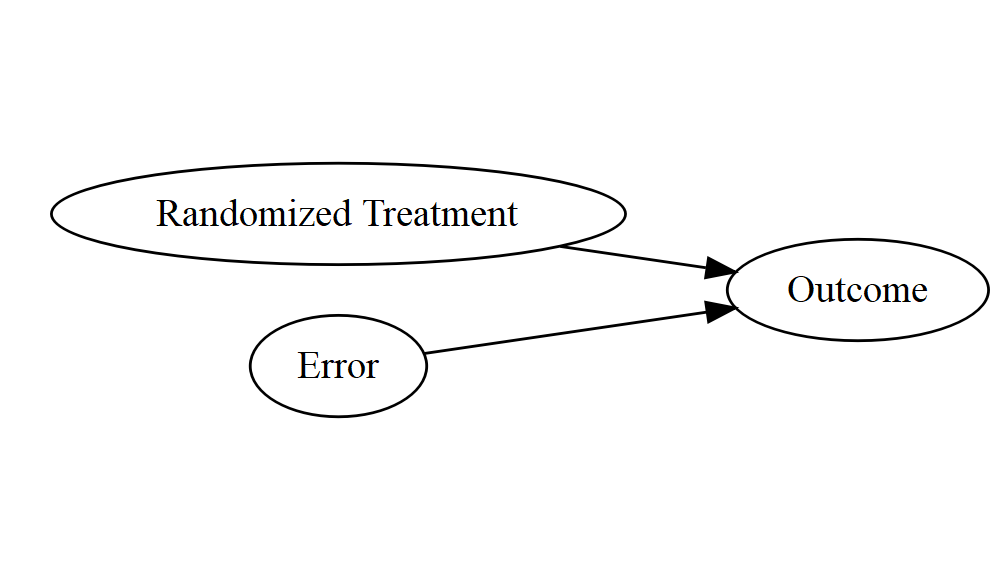
\includegraphics[width=\maxwidth]{figure/explanation1-1} 

\end{knitrout}
\end{frame}

\begin{frame}
\frametitle{Randomization}
\begin{itemize}
\item Why does randomization remove selection bias?
\pause
\item Assume: $Y_{1i} = Y_{0i} + \alpha$, where $\alpha$ is the real constant treatment effect
\pause
\end{itemize}
$$ \hat{ATE} = E(Y_1|D=1) - E(Y_0|D=0)$$ \\ \pause
$$ \hat{ATE} = E(Y_0+\alpha|D=1) - E(Y_0|D=0)$$ \\ \pause
$$ \hat{ATE} = \underbrace{\alpha}_\text{Real ATE} + \underbrace{E(Y_0|D=1) - E(Y_0|D=0)}_\text{Bias}$$ \\
\pause
\begin{itemize}
\item Now, use the Independence of Treatment Assignment:
\end{itemize}
$$ E(Y_0|D=1) = E(Y_0|D=0)$$ \\ \pause
$$ \hat{ATE} = \underbrace{\alpha}_\text{Real ATE} $$ \\
\pause
\begin{itemize}
\item This works for observable \textit{and} unobservable influences
\end{itemize}
\end{frame}

\begin{frame}
\frametitle{Randomization}
\begin{itemize}
\item But this logic works only based on \textbf{expectations} (averages)
\pause
\begin{itemize}
\item \textit{On average}, potential outcomes will be balanced
\pause
\item That's more likely in larger samples
\pause
\item Less likely in small samples; by chance, potential outcomes may be biased
\pause
\item We have no way of \textit{verifying} if potential outcomes are biased
\end{itemize}
\end{itemize}
\end{frame}

\begin{frame}
\frametitle{Balance in Randomized Experiments}
\begin{multicols}{2}
\begin{itemize}
\item Balance on potential outcomes is unlikely in small samples
\end{itemize}
\columnbreak
\pause
N=10
\begin{knitrout}
\definecolor{shadecolor}{rgb}{0.969, 0.969, 0.969}\color{fgcolor}
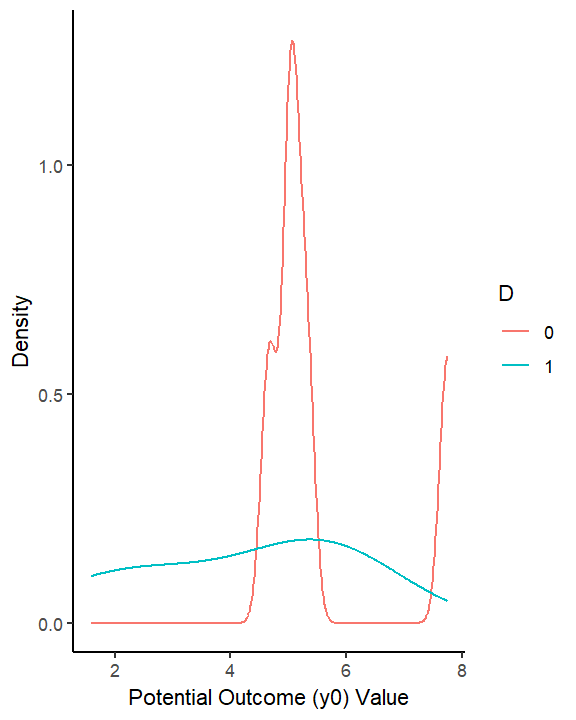
\includegraphics[width=\maxwidth]{figure/balance_N1-1} 

\end{knitrout}
\end{multicols}
\end{frame}

\begin{frame}
\frametitle{Balance in Randomized Experiments}
\begin{multicols}{2}
\begin{itemize}
\item Balance on potential outcomes is unlikely in small samples
\item But the Law of Large Numbers helps us in large samples
\end{itemize}
\columnbreak
N=20
\begin{knitrout}
\definecolor{shadecolor}{rgb}{0.969, 0.969, 0.969}\color{fgcolor}
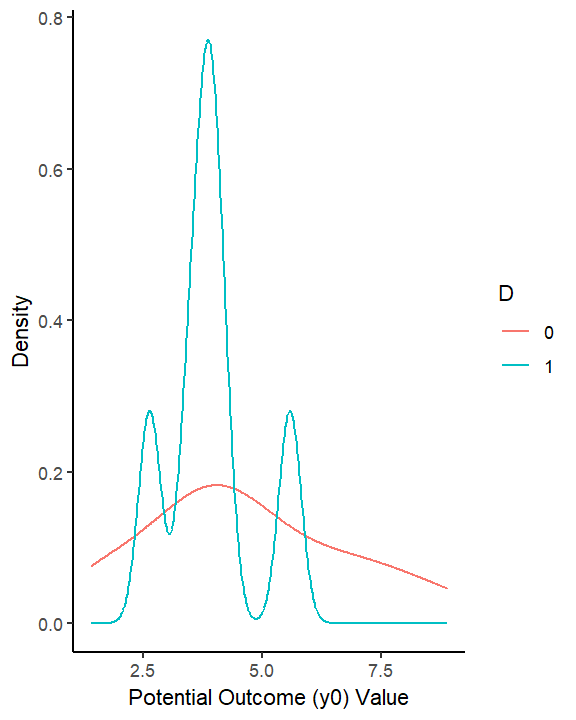
\includegraphics[width=\maxwidth]{figure/balance_N2-1} 

\end{knitrout}
\end{multicols}
\end{frame}

\begin{frame}
\frametitle{Balance in Randomized Experiments}
\begin{multicols}{2}
\begin{itemize}
\item Balance on potential outcomes is unlikely in small samples
\item But the Law of Large Numbers helps us in large samples
\end{itemize}
\columnbreak
N=50
\begin{knitrout}
\definecolor{shadecolor}{rgb}{0.969, 0.969, 0.969}\color{fgcolor}
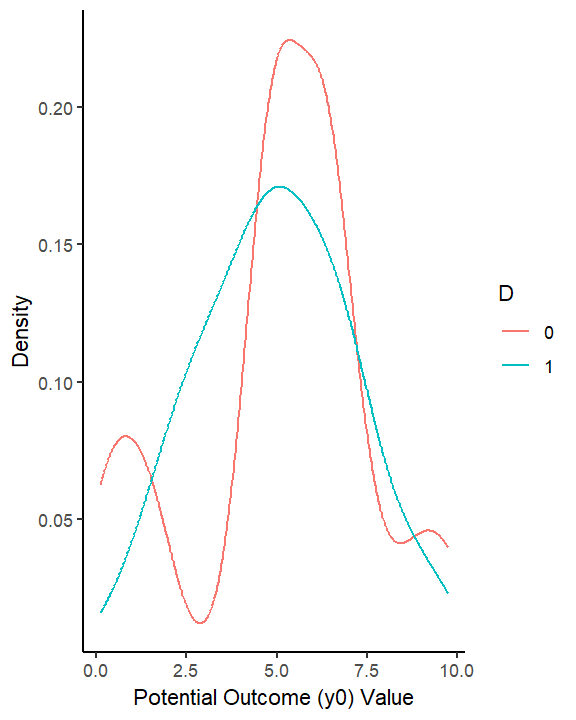
\includegraphics[width=\maxwidth]{figure/balance_N4-1} 

\end{knitrout}
\end{multicols}
\end{frame}

\begin{frame}
\frametitle{Balance in Randomized Experiments}
\begin{multicols}{2}
\begin{itemize}
\item Balance on potential outcomes is unlikely in small samples
\item But the Law of Large Numbers helps us in large samples
\end{itemize}
\columnbreak
N=100
\begin{knitrout}
\definecolor{shadecolor}{rgb}{0.969, 0.969, 0.969}\color{fgcolor}
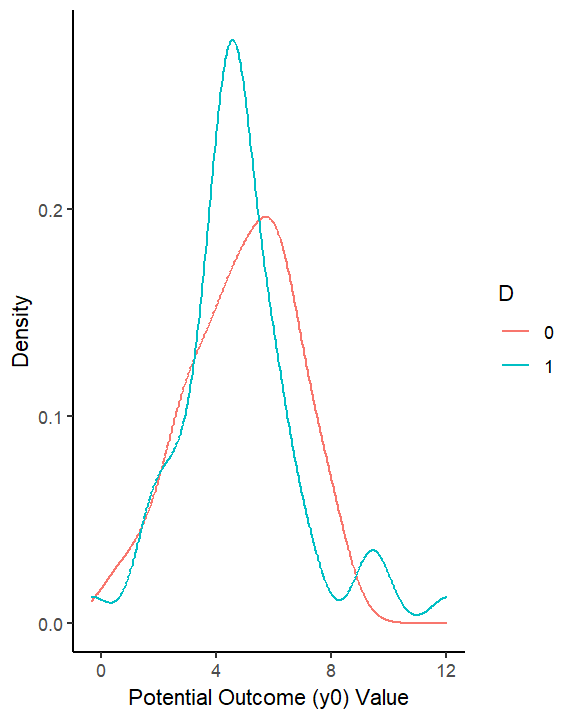
\includegraphics[width=\maxwidth]{figure/balance_N5-1} 

\end{knitrout}
\end{multicols}
\end{frame}

\begin{frame}
\frametitle{Balance in Randomized Experiments}
\begin{multicols}{2}
\begin{itemize}
\item Balance on potential outcomes is unlikely in small samples
\item But the Law of Large Numbers helps us in large samples
\end{itemize}
\columnbreak
N=1000
\begin{knitrout}
\definecolor{shadecolor}{rgb}{0.969, 0.969, 0.969}\color{fgcolor}
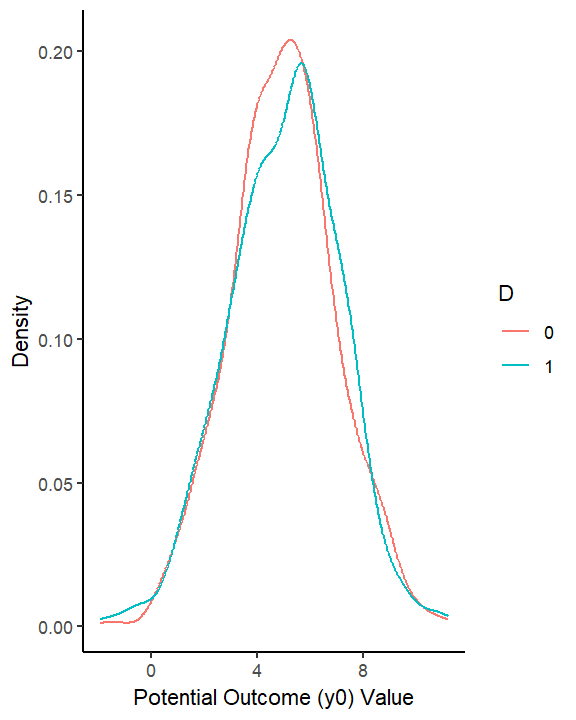
\includegraphics[width=\maxwidth]{figure/balance_N6-1} 

\end{knitrout}
\end{multicols}
\end{frame}

\begin{frame}
\frametitle{Balance in Randomized Experiments}
\begin{multicols}{2}
\begin{itemize}
\item Balance on potential outcomes is unlikely in small samples
\item But the Law of Large Numbers helps us in large samples
\end{itemize}
\columnbreak
N=100000
\begin{knitrout}
\definecolor{shadecolor}{rgb}{0.969, 0.969, 0.969}\color{fgcolor}
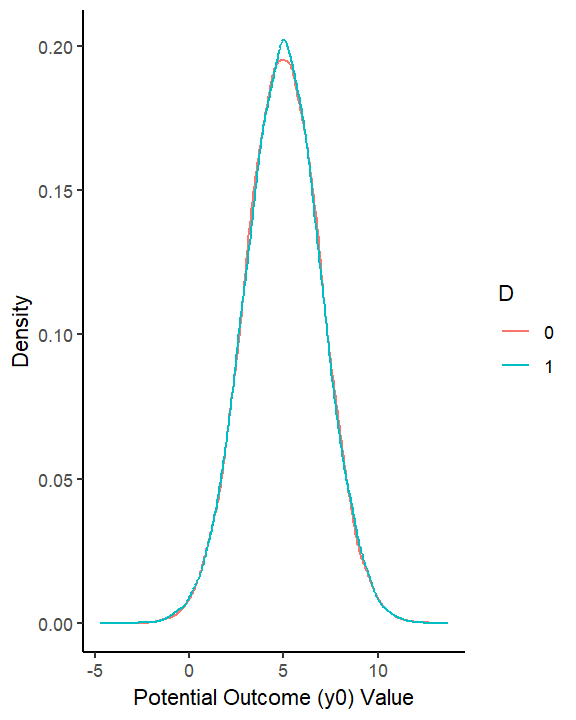
\includegraphics[width=\maxwidth]{figure/balance_N7-1} 

\end{knitrout}
\end{multicols}
\end{frame}

\section{Analysis}

\begin{frame}
\frametitle{Analyzing Field Experiments}
\begin{itemize}
\item If treatment is random we know that:
\begin{eqnarray}
\hat{ATE} &= E(Y_1|D=1) - E(Y_0|D=0) \\
& = E(Y_1) - E(Y_0) \\
& = \text{Real ATE}
\end{eqnarray}
\pause
\item What is $E(Y_1|D=1)$? 
\pause 
\item What is $E(Y_0|D=0)$?
\pause
\item This is easy! 
\pause
\item Just the difference in outcome means between treatment and control units
\pause
\begin{itemize}
\item And a simple T-test for statistical significance
\pause
\item \textbf{NO modelling assumptions} (``non-parametric'')
\end{itemize}
\end{itemize}
\end{frame}

\begin{frame}
\frametitle{Analyzing Field Experiments}
\begin{itemize}
\item Simple Regression $=$ Difference-in-means T-test
\pause
\item By definition: 
$$Y^{obs}_i = Y_{0i}(1-D_i) + Y_{1i}D_i$$
$$Y^{obs}_i = Y_{0i} + (Y_{1i} - Y_{0i}) D_i$$
\pause
\item We can estimate:
$$Y^{obs}_i = \alpha + \beta D_i + \epsilon_i$$
\pause
\item So:
$$\hat{\beta} = E(Y_{1i} - Y_{0i})$$
\end{itemize}
\end{frame}

\begin{frame}
\frametitle{Analyzing Field Experiments}
\begin{itemize}
\item Simple Regression is \textbf{identical} to a Difference-in-means T-test
\footnotesize
\item T-test Results:
% latex table generated in R 3.5.2 by xtable 1.8-3 package
% Fri Mar 29 10:11:31 2019
\begin{table}[ht]
\centering
\begin{tabular}{rrrr}
  \hline
 & estimate & statistic & p.value \\ 
  \hline
1 & 0.27065 & 2.69475 & 0.00706 \\ 
   \hline
\end{tabular}
\end{table}

\pause
\item Regression Results ($Y_i = \alpha + \beta D_i + \epsilon_i$):
% latex table generated in R 3.5.2 by xtable 1.8-3 package
% Wed Apr 03 16:23:27 2019
\begin{table}[ht]
\centering
\begin{tabular}{rlrrrr}
  \hline
 & term & estimate & std.error & statistic & p.value \\ 
  \hline
1 & (Intercept) & 0.03459 & 0.07110 & 0.48647 & 0.62664 \\ 
  2 & treatment & 0.27065 & 0.10044 & 2.69472 & 0.00706 \\ 
   \hline
\end{tabular}
\end{table}

\end{itemize}
\normalsize
\end{frame}

\begin{frame}
\frametitle{Repeated Experiments}
\begin{multicols}{2}
\begin{itemize}
\item The results from one experiment are not perfect
\pause
\item Estimated treatment effects are still \textit{probabilistic} (random variables) so we may get the wrong answer by chance
\pause
\item In repeated experiments, 95\% of confidence intervals will cross the true treatment effect
\pause
\item \href{https://poliong.shinyapps.io/to_deploy/}{Try repeated experiments in an App}
\pause
\end{itemize}
\columnbreak
\begin{knitrout}
\definecolor{shadecolor}{rgb}{0.969, 0.969, 0.969}\color{fgcolor}
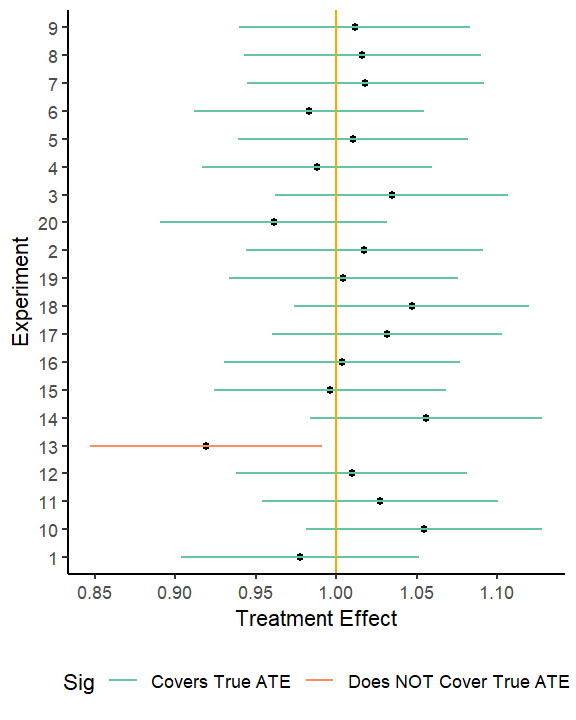
\includegraphics[width=\maxwidth]{figure/repeated_exp-1} 

\end{knitrout}
\end{multicols}
\end{frame}

\begin{frame}
\frametitle{Clustered Treatments}
\begin{itemize}
\item Clustered sampling: To reduce data collection costs
\pause
\item Clustered treatment: To reduce implementation costs, or to test specific theories
\pause
\begin{itemize}
\item Eg. Holding Town Hall meetings does not make sense at the individual level
\end{itemize}
\pause
\item If treatment (or sampling) are clustered, we will have \textit{dependencies} in our errors - closer people are more similar
\pause
\item So \textbf{standard errors must be clustered at the level of treatment/sampling} (eg. villages)
\pause
\item In general, causal inference is more efficient with more higher-level units (more villages, less people per village)
\pause
\begin{itemize}
\item But there is usually a cost trade-off
\end{itemize}
\end{itemize}
\end{frame}

\begin{frame}
\frametitle{Controlling for Covariates}
\begin{itemize}
\item Do we need to control for covariates in experiments?
\pause
\item If randomization worked and the sample size is large, usually not
\pause
\item Three reasons to include controls:
\begin{enumerate}
\item \textbf{Small sample}, but note causal inference is now model-dependent
\pause
\item \textbf{Chance/residual imbalance} on a specific variable which we want to adjust for
\pause
\item \textbf{To improve precision}, i.e. reduce the standard errors on $\beta$
\begin{itemize}
\item The more variation in $Y$ we can explain with covariates, the more certain we can be on the effect of $D$
\end{itemize}
\end{enumerate}
\end{itemize}
\end{frame}

\begin{frame}
\frametitle{Other Quantities of Interest}
\begin{itemize}
\item Average Treatment Effects are just one summary statistic
\begin{itemize}
\item Treatment effects are not normally constant
\pause
\item Averages can be influenced by outliers
\end{itemize}
\pause
\item What if an average effect of +5\% income leaves half the population hugely rich and half very poor?
\pause
\item Average treatment effects are easiest (difference-in-means equals mean-difference)
\pause
\item But we can also estimate Quantile treatment effects, eg. the effect of treatment on the bottom 10\% of the distribution
\end{itemize}
\end{frame}

\begin{frame}
\frametitle{Other Quantities of Interest}
\begin{multicols}{2}
\begin{itemize}
\item Assume the treatment effect is normally-distributed: $N(\mu=1,\sigma^2=1)$
\end{itemize}
\pause
\columnbreak
\begin{knitrout}
\definecolor{shadecolor}{rgb}{0.969, 0.969, 0.969}\color{fgcolor}
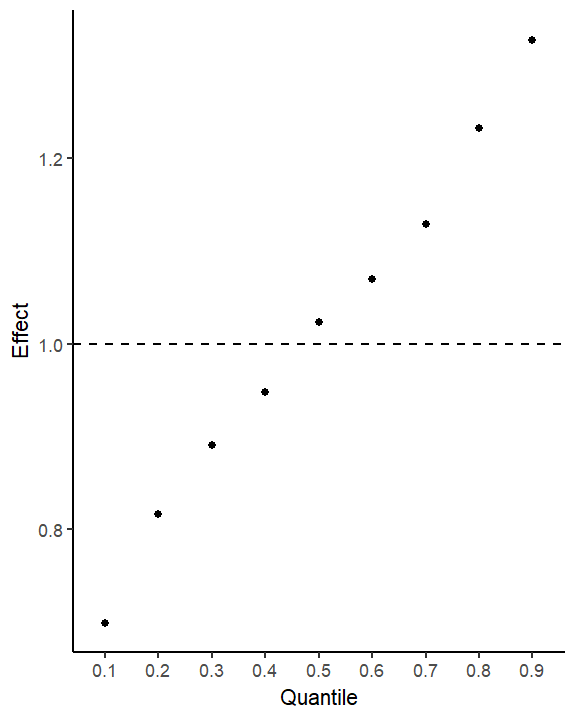
\includegraphics[width=\maxwidth]{figure/quant_reg-1} 

\end{knitrout}
\end{multicols}
\end{frame}

\begin{frame}
\frametitle{Heterogeneous Effects}
\begin{itemize}
\item \textbf{Experiment:} We place a new health centre in half of all communities at random, and want to measure whether the health centre has a bigger effect in poor or rich neighbourhoods
\pause
\item \textbf{Analysis:} Run a single regression with an interaction between treatment and neighbourhood income
\pause
\item \textbf{Result:} The health centre boosts health by 20\% in rich neighbourhoods and reduces health in poor neighbourhoods by 20\%
\pause
\item \textbf{Interpretation:} Does neighbourhood poverty cause health centres to have a negative impact?  
\begin{itemize}
\pause
\item We cannot interpret the 'moderator' variable as having a causal effect, the different treatment effects could be due to omitted variables or selection
\pause
\item Only the health centre was randomly assigned, not neighbourhood income!
\end{itemize}
\end{itemize}
\end{frame}

\section{Assumptions}

\begin{frame}
\frametitle{Assumptions}
\begin{enumerate}
\item Compliance with Randomization procedure
\pause
\item Randomization produced balance on potential outcomes
\pause
\item No Spillovers (SUTVA)
\pause
\item Excludability
\pause
\end{enumerate}
\end{frame}

\begin{frame}
\frametitle{1. Compliance with Randomization procedure}
\begin{itemize}
\item Randomization is unpopular, political, and sometimes resisted
\pause
\item Need to verify treatment allocation
\begin{itemize}
\item Transparency, documentation
\end{itemize}
\pause
\item And treatment compliance
\begin{itemize}
\item Did anyone assigned to control manage to get treatment?
\item Did anyone assigned to treatment refuse?
\pause
\end{itemize}
\item \textbf{Design:} Double-blind assignment
\pause
\item \textbf{Checks:} Qualitative fieldwork
\pause
\item \textbf{Analysis:} More on how to respond to non-compliance next week
\end{itemize}
\end{frame}

\begin{frame}
\frametitle{2. Randomization Produced Balanced Potential Outcomes}
\begin{itemize}
\item Impossible to Test!
\pause
\item But we can test observable pre-treatment covariates
\pause
\item If covariates are the same in the treatment and control groups, this variable \textit{cannot} explain any differences in outcomes
\pause
\item If lots of variables are balanced, it's likely potential outcomes are too
\pause
\item \textbf{Check:} Normally a difference in means T-test of covariates between treatment and control groups
\pause
\item \textbf{Check:} Or a Kolmogorov-Smirnov (KS) Test of identical distributions
\end{itemize}
\end{frame}

\begin{frame}
\frametitle{2. Randomization Produced Balanced Potential Outcomes}
\begin{itemize}
\item What if a balance test comes back with a p-value < 0.05?
\pause
\item It probably will!
\begin{enumerate}
\item We are testing many variables, so some differences arise by chance
\pause
\item We have a large N, so we can detect very small differences
\pause
\end{enumerate}
\item \textbf{Check:} For balance, what matters are \textit{substantive} differences, not so much p-values
\pause
\item Two safety nets:
\begin{enumerate}
\item \textbf{Analysis:} We can still include covariates in our analysis, controlling for 'residual' imbalance
\pause
\item \textbf{Analysis:} We are using p-values in our \textit{analysis}, which take into account 'chance' imbalance
\pause
\end{enumerate}
\end{itemize}
\end{frame}

\begin{frame}
\frametitle{3. SUTVA}
\begin{itemize}
\item Stable Unit Treatment Value Assumption = \textbf{No Spillovers}
\pause
\item Technically, treatment of unit $j$ does not affect the potential outcomes for unit $i$
\pause
$$(Y_{1i}, Y_{0i}) \perp D_j$$
\pause
$$Y_i(D_i, D_j, D_k, D_l, D_m, D_n, D_o, D_p...) = Y_i(D_i)$$
\pause
\item Spillovers interfere with our control group, so the comparison does not measure the direct effect of a treatment on person $i$ 
\pause
\item But spillovers are common! If you get an award, I might feel more motivated or less motivated
\pause
\item What should we do?
\pause
\begin{itemize}
\item \textbf{Design:} Limit risk of spillovers, eg. leave 20 miles between each unit in sampling
\item \textbf{Check:} Qualitative fieldwork
\item \textbf{Analysis:} Try to \textit{measure} spillovers
\end{itemize}
\end{itemize}
\end{frame}

\begin{frame}
\frametitle{4. Excludability}
\begin{itemize}
\item \textbf{Nothing else correlated with treatment affects potential outcomes}
\pause
\item Assignment to treatment causes a \textbf{'parallel'} treatment
\pause
\begin{itemize}
\item Eg. We decide to share information about specific politicians on the radio, but the politicians find out and counter with their own broadcasts
\end{itemize}
\pause
\item Our treatment effect is no longer \textit{only} the effect of our information intervention
\pause
\item ...Or do we want to measure these additional effects?
\end{itemize}
\end{frame}

\begin{frame}
\frametitle{4. Excludability}
\begin{itemize}
\item Distinguish between the downstream consequences of treatment and 'parallel' treatments
\end{itemize}
\pause
\footnotesize
\begin{multicols}{2}
\textbf{Downstream ('net') Consequences}
\begin{itemize}
\pause
\item Eg. We give a cash handout to families, and then they also start paying taxes; which explains their changing attitudes to government?
\pause
\item We find zero effect of government investing \$1000 in healthcare on health outcomes, because households responded by reducing their spending by exactly \$1000
\end{itemize}
\columnbreak
\pause
\textbf{Parallel Treatments}
\begin{itemize}
\pause
\item Eg. Measurement bias: Researchers give treated units 'the benefit of the doubt' and record higher outcomes for them
\pause
\item Or Hawthorne Effects: Participants respond to being studied, not treatment (more next week)
\end{itemize}
\end{multicols}
\normalsize
\begin{itemize}
\pause
\item \textbf{Design:} Careful specification of treatment and control
\end{itemize}
\end{frame} 

\begin{frame}
\frametitle{4. Excludability}
\begin{multicols}{2}
Downstream Consequence of Treatment
\begin{knitrout}
\definecolor{shadecolor}{rgb}{0.969, 0.969, 0.969}\color{fgcolor}
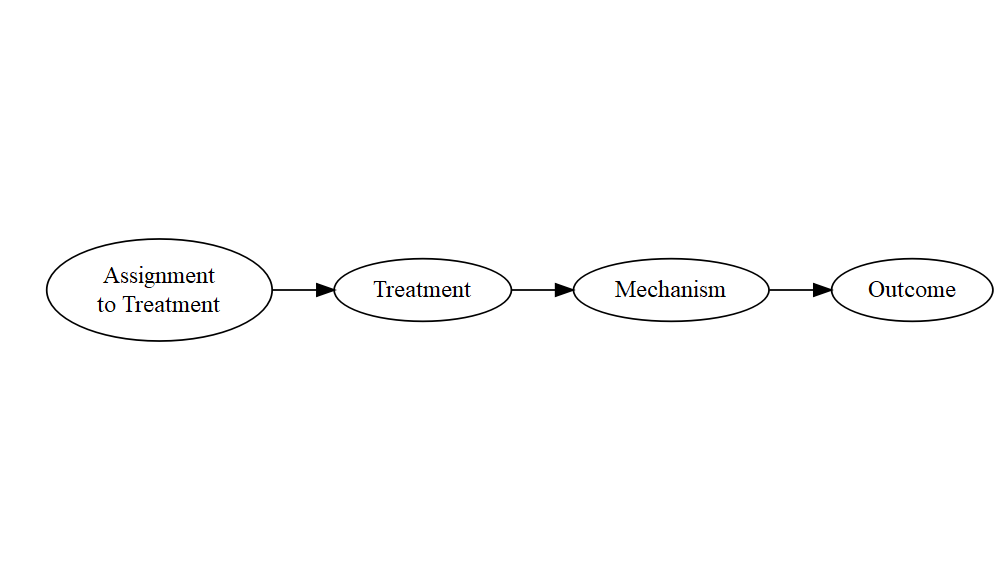
\includegraphics[width=\maxwidth]{figure/Excludability1-1} 

\end{knitrout}
\columnbreak
\pause
Parallel Treatment
\begin{knitrout}
\definecolor{shadecolor}{rgb}{0.969, 0.969, 0.969}\color{fgcolor}
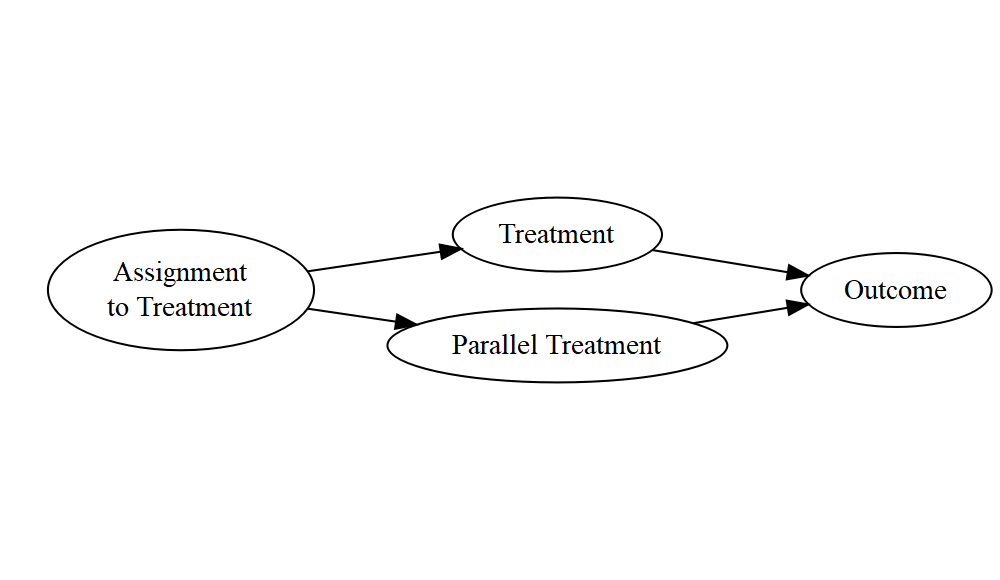
\includegraphics[width=\maxwidth]{figure/Excludability2-1} 

\end{knitrout}
\end{multicols}
\end{frame}

\section{Implementation}

\begin{frame}
\frametitle{Implementing Field Experiments}
\begin{itemize}
\item How do we randomize?
\begin{itemize}
\item Hard! We can't just 'pick' treated units off the top of our heads
\pause
\item Computers are deterministic
\pause
\item The best we can do is to use atmospheric noise or radioactive decay
\pause
\end{itemize}
\item In the real world, randomization is hard
\begin{itemize}
\item Pressure to help the most needy
\pause
\item Political pressure
\pause
\item We don't want to be guinea pigs!
\end{itemize}
\end{itemize}
\end{frame}


\begin{frame}
\frametitle{Implementing Field Experiments}
\begin{itemize}
\item How do we randomize?
\pause
\item Three options to assign treatment and control 'independent' of potential outcomes:
\pause
\begin{itemize}
\item We have N units and want equal probability of treatment for each:
\end{itemize}
\begin{enumerate}
\item Flip a coin for every unit so every unit has probability $0.5$ of treatment
\pause
\item Randomize the order of the units and assign the first $\frac{N}{2}$ units to treatment
\pause
\item Pair similar units and flip a coin to assign one from each pair to treatment
\pause
\end{enumerate}
\item What's the difference between these three options?
\pause
\item What \% treated? 50:50 is usually most efficient
\pause
\item To actually randomize, use the \href{https://cran.r-project.org/web/packages/randomizr/vignettes/randomizr_vignette.html}{`randomizr' package} 
\end{itemize}
\end{frame}

\begin{frame}
\frametitle{Implementing Field Experiments}
\begin{itemize}
\item \textbf{Blocking}
\pause
\item Randomization is \textit{inefficient} and risky
\pause
\item We know we need balance on key covariates, eg. gender, so why leave this to chance??
\begin{itemize}
\item 
\pause
\item We can measure these variables and \textit{enforce} balance (50\% female in both treatment and control)
\pause
\item Blocking means randomizing \textit{within} fixed groups
\pause
\item Eg. We have a sample size of 4000, half male, half female
\pause
\begin{multicols}{2}
Without Blocking:
\begin{table}[]
\begin{tabular}{|l|l|l|}
\hline
        & M    & F    \\ \hline
Treated & 1042 & 958  \\ \hline
Control & 972  & 1028 \\ \hline
\end{tabular}
\end{table}
\columnbreak
With Blocking:
\begin{table}[]
\begin{tabular}{|l|l|l|}
\hline
        & M    & F    \\ \hline
Treated & 1000 & 1000  \\ \hline
Control & 1000 & 1000 \\ \hline
\end{tabular}
\end{table}
\end{multicols}
\end{itemize}
\pause
\item "Block what you can; randomize what you cannot"
\pause
\item We focus on within-block variation: $Y_i = \alpha + D_i + B_i + \epsilon_i$
\end{itemize}
\end{frame}

\begin{frame}
\frametitle{Implementing Field Experiments}
\begin{itemize}
\item Random treatment vs. Random samples
\end{itemize}
\begin{multicols}{2}
\textbf{Random Treatment}
\begin{itemize}
\pause
\item Representative potential outcomes
\pause
\item \textit{Causal} Inference
\end{itemize}
\columnbreak
\textbf{Random Samples}
\begin{itemize}
\pause
\item Sample representative of larger population
\pause
\item \textit{Statistical} Inference
\end{itemize}
\end{multicols} 
\pause
\begin{itemize}
\item Both work in the same way - randomization avoids selection (into the data/treatment)
\end{itemize}
\end{frame}

\section{Critiquing}

\begin{frame}
\frametitle{Critiquing Field Experiments}
\begin{itemize}
\item Field experiments are easy to evaluate. What can go wrong??
\end{itemize}
\end{frame}

\begin{frame}
\frametitle{1. Results are a Black Box}
\begin{itemize}
\item We know that $D$ causes $Y$ in this population. \pause So what? What did we learn about political science?
\pause
\begin{itemize}
\item We know that giving citizens health insurance makes them more likely to vote. \pause Why?? How?? What is the mechanism?
\pause
\item Due to increased wealth? Increased trust in government? More mobility?
\end{itemize}
\pause
\item What theory is this testing? \pause Does it reject any theory?
\pause
\item We want to test theories, not treatments
\end{itemize}
\end{frame}

\begin{frame}
\frametitle{2. Generalizability of Context}
\begin{itemize}
\item Our causal conclusions are \textbf{restricted to the population we drew our sample from}
\pause
\item Income makes attitudes to redistribution more negative in the USA
\pause
\begin{itemize}
\item What is the effect in Angola?
\end{itemize}
\pause
\item Secondary school education leads to more conservative voting
\pause
\begin{itemize}
\item What is the effect of university education?
\end{itemize}
\pause
\item Yes, you randomly sampled and randomly assigned treatment, but not in the full population we want to learn about
\pause
\begin{itemize}
\item The places that agree to field experiments are not representative
\end{itemize}
\end{itemize}
\end{frame}

\begin{frame}
\frametitle{3. Generalizability of Treatment}
\begin{itemize}
\item The effect of an education intervention in an experiment in Butant\~{a} raised test scores by 20\%, and was evaluated and verified by USP
\pause
\item The government expands the program nationwide. Do Brazilian students' scores improve on average by 20\%?
\pause
\item Three problems:
\begin{enumerate}
\item \textbf{Implementation Varies:} Implementing at scale is \textbf{hard}, costly and requires delegation to less motivated and skilled actors.
\pause
\item \textbf{Ownership and Excludability:} 
\begin{itemize}
\item Telling someone to implement an intervention is different from working with a self-motivated actor who designed the intervention. 
\pause
\item Knowing you were randomly assigned to treatment rather than choosing treatment changes political ownership, perceptions and motivation.
\end{itemize}
\pause
\item \textbf{General Equilibrium Effects:} Average test scores went from 70\% to 90\%, so the exam board readjusted the test and made it harder.
\end{enumerate}
\end{itemize}
\end{frame}

\begin{frame}
\frametitle{3. Generalizability of Treatment}
\begin{itemize}
\item Eg. The Millennium Villages Project
\pause
\item WB/UN/Columbia University tried to invest USD\$120 per person in 14 African villages
\pause
\item Mixed but positive results: crop yields increased 85-350\%, malaria reduced 50\% compared to controls
\pause
\item But:
\begin{enumerate}
\item Sites were not representative (close to main roads and cities so they're easy to visit)
\pause
\item Treatment could not be scaled (Every village cannot get visits from Columbia professors twice a year)
\pause
\item And politics was ignored (No implementation unless you give locals responsibility, but then you lose control)
\end{enumerate}
\end{itemize}
\end{frame}

\begin{frame}
\frametitle{4. Skewed Learning}
\begin{itemize}
\item Research focuses on where experiments are most \textit{possible}, not where it is most needed
\pause
\item Selection bias in research findings
\end{itemize}
\end{frame}


\end{document}

% Balance tests really unnecessary as p-values already take chance of bad randomisation into account (https://janhove.github.io/reporting/2014/09/26/balance-tests)
% 95% interval repeated experiments example
% *Deworming wars - As example of difficulty of interpreting and aggregating field experiments

% Outcomes defined over time; large effects decay
% Downstream experiments
% Heterogeneous treatment effects
% Non-compliance, attrition


% Give examples of bad designs and get them to identify why
%Data-mining on heterog effects - need to justify by theory. Eg. treated five villages and worked in one - do we believe it?
% GE effects, eg. changes in sorting, competition, expectations, norms
%Hawthorne effects (for next week)
% Venn diagram style explanation of popn, sample, treated and control


%setwd('C:\\Users\\Jonny\\Google Drive\\Academic\\USP\\Class\\Week 1 - Intro\\Lecture Slides')
%knitr::knit("Slides_Wk1_intro_5.Rnw")
